\documentclass[12pt,a4paper]{article}
\usepackage[top=1.2cm,bottom=1.2cm,left=1.7cm,right=1.7cm]{geometry}
\usepackage{graphicx}
\usepackage{amsmath}
\usepackage{hyperref}
\usepackage{array}

% --- spacing ---
\setlength{\parskip}{2pt}
\setlength{\parindent}{0pt}
\setlength{\abovecaptionskip}{2pt}
\setlength{\belowcaptionskip}{0pt}
\setlength{\floatsep}{3pt}
\setlength{\textfloatsep}{3pt}

% --- compact sections ---
\makeatletter
\renewcommand\section{\@startsection{section}{1}{\z@}%
  {4pt \@plus 1pt \@minus 1pt}{2pt}%
  {\normalfont\normalsize\bfseries}}
\makeatother

\begin{document}

\begin{center}
{\large\textbf{Urban Microbiome Composition and Economic Development:\\A Multi-Cohort Metagenomic Analysis}}\\[2pt]
\end{center}

% ============================================================
\section*{Research Question}

Does economic development (high-income (further referenced as HIC) vs.\ upper-middle-income (further referenced as UMIC) countries)
influence urban environmental microbiome composition, and do these differences persist after controlling for geographic confounders and study-level batch effects?\\
\textbf{Hypothesis:}
The level of economic development influences the urban microbiome diversity,
with higher-income cities hosting specialized microbial communities shaped by the factors of
industrial pollution, sanitation and agricultural land use.

% ============================================================
\section*{Data}
\textbf{Database:} SPIRE Environmental Metagenomics (MetaPhlAn4 species profiles; total: 26938 samples, 391 studies; urban biome subset: 1909 samples)\\
\textbf{Stage 1:} 1417 urban samples (HIC: USA+Denmark+Singapore $n=1247$; UMIC: China $n=170$); 561 species after prevalence filtering; Centered Log-Ratio transformation; geographic confounders identified.\\
\textbf{Stage 2:} 135 samples with complete metadata (USA $n=29$, China $n=106$); 134 species; linear regression with/without geographic covariates.\\
\textbf{Stage 3:} 6 independent cohorts, $n=1258$ (HIC 1152, UMIC 106), 104 species observed in outdoor air, indoor dust, sewage, and vehicle surfaces.\\

\begin{table}[h!]
\centering
\small
\setlength{\tabcolsep}{5pt}
\begin{tabular}{lllll}
\hline
\textbf{Study} & \textbf{Country} & \textbf{Income} & \textbf{Material} & \textbf{n} \\
\hline
Gusareva 2019 & Singapore & HIC & Outdoor air & 388 \\
Ohara 2017 & USA & HIC & Vehicle surfaces & 398 \\
Brinch 2020 & Denmark & HIC & Sewage & 216 \\
Fahimipour 2018 & USA & HIC & Indoor dust & 115 \\
Qin 2020 & China & UMIC & Outdoor air & 106 \\
Shaffer 2021 & USA & HIC & Mixed urban & 35 \\
\hline
\multicolumn{5}{l}{\small Table 1: Cohorts chosen for meta-analysis}
\end{tabular}
\end{table}

% ============================================================
\section*{Results}

\textbf{Stage 1: Diversity analysis.}
UMIC samples had significantly higher richness (71.6 vs.\ 51.1, $p<10^{-6}$), Shannon (2.04 vs.\ 1.36, $p<10^{-7}$), and Simpson (0.60 vs.\ 0.50, $p<10^{-5}$) diversity.
PCA revealed community-level separation (PC1 = 21.7\%).
529/561 species identified as differentially abundant (FDR $q<0.05$, Mann-Whitney U test): 124 UMIC-enriched, 405 HIC-enriched.

\textbf{Stage 2: MWAS with covariate adjustment.}
Geographic variables were major confounders (longitude and elevation with $p<10^{-3}$).
Unadjusted analysis flagged 64.2\% of species; after adjusting for latitude and elevation, 74.6\% of species retained robust economic associations (FDR $q<0.05$),
demonstrating that economic effects are real but substantially confounded by geography.

\textbf{Stage 3: Multi-cohort meta-analysis.}
\textbf{Batch effects:} Strong study-level clustering (Kruskal-Wallis H=634, $p<10^{-100}$; Spearman $r_{\text{study}}=-0.53$). Ordinary least square residualization (per-species regression on study dummies; residuals retained as corrected values) reduced batch correlation to $r_{\text{study}}=0.09$.\\
\textbf{Pooled analysis} (Centered log ratio $\sim$ Income + Study, all 6 cohorts): only 8/104 species survived FDR correction, as differences in sample material (air vs.\ sewage vs.\ dust vs.\ vehicle surfaces) drive stronger compositional shifts than economic group.\\
\textbf{Air-cohort comparison} (Gusareva Singapore vs.\ Qin China): as both studies sampled outdoor air but in different income-group countries, comparing them isolates the economic signal from the sample-type confound. Outcome: 91/104 species differentially abundant (FDR $q<0.05$; 63 HIC-enriched, 28 UMIC-enriched).\\
\textbf{Alpha diversity (air cohorts):} UMIC Shannon $0.74\pm0.29$ vs.\ HIC $0.43\pm0.47$ ($p=6.8\times10^{-13}$); UMIC richness $39.8\pm22.6$ vs.\ HIC $2.2\pm2.8$ ($p=3.4\times10^{-56}$) — measured across 104 overlap species.\\

% ============================================================
\section*{Conclusions}
Economic development significantly influences urban microbiome diversity across all three analyses.
However, sample-type heterogeneity across independent cohorts creates strong batch effects that mask biological signal in pooled analyses.
Matching by sample material (air cohorts) recovers 91 significant species, validating the covariate-adjusted results from Stage 2.

\begin{figure}[h!]
\centering
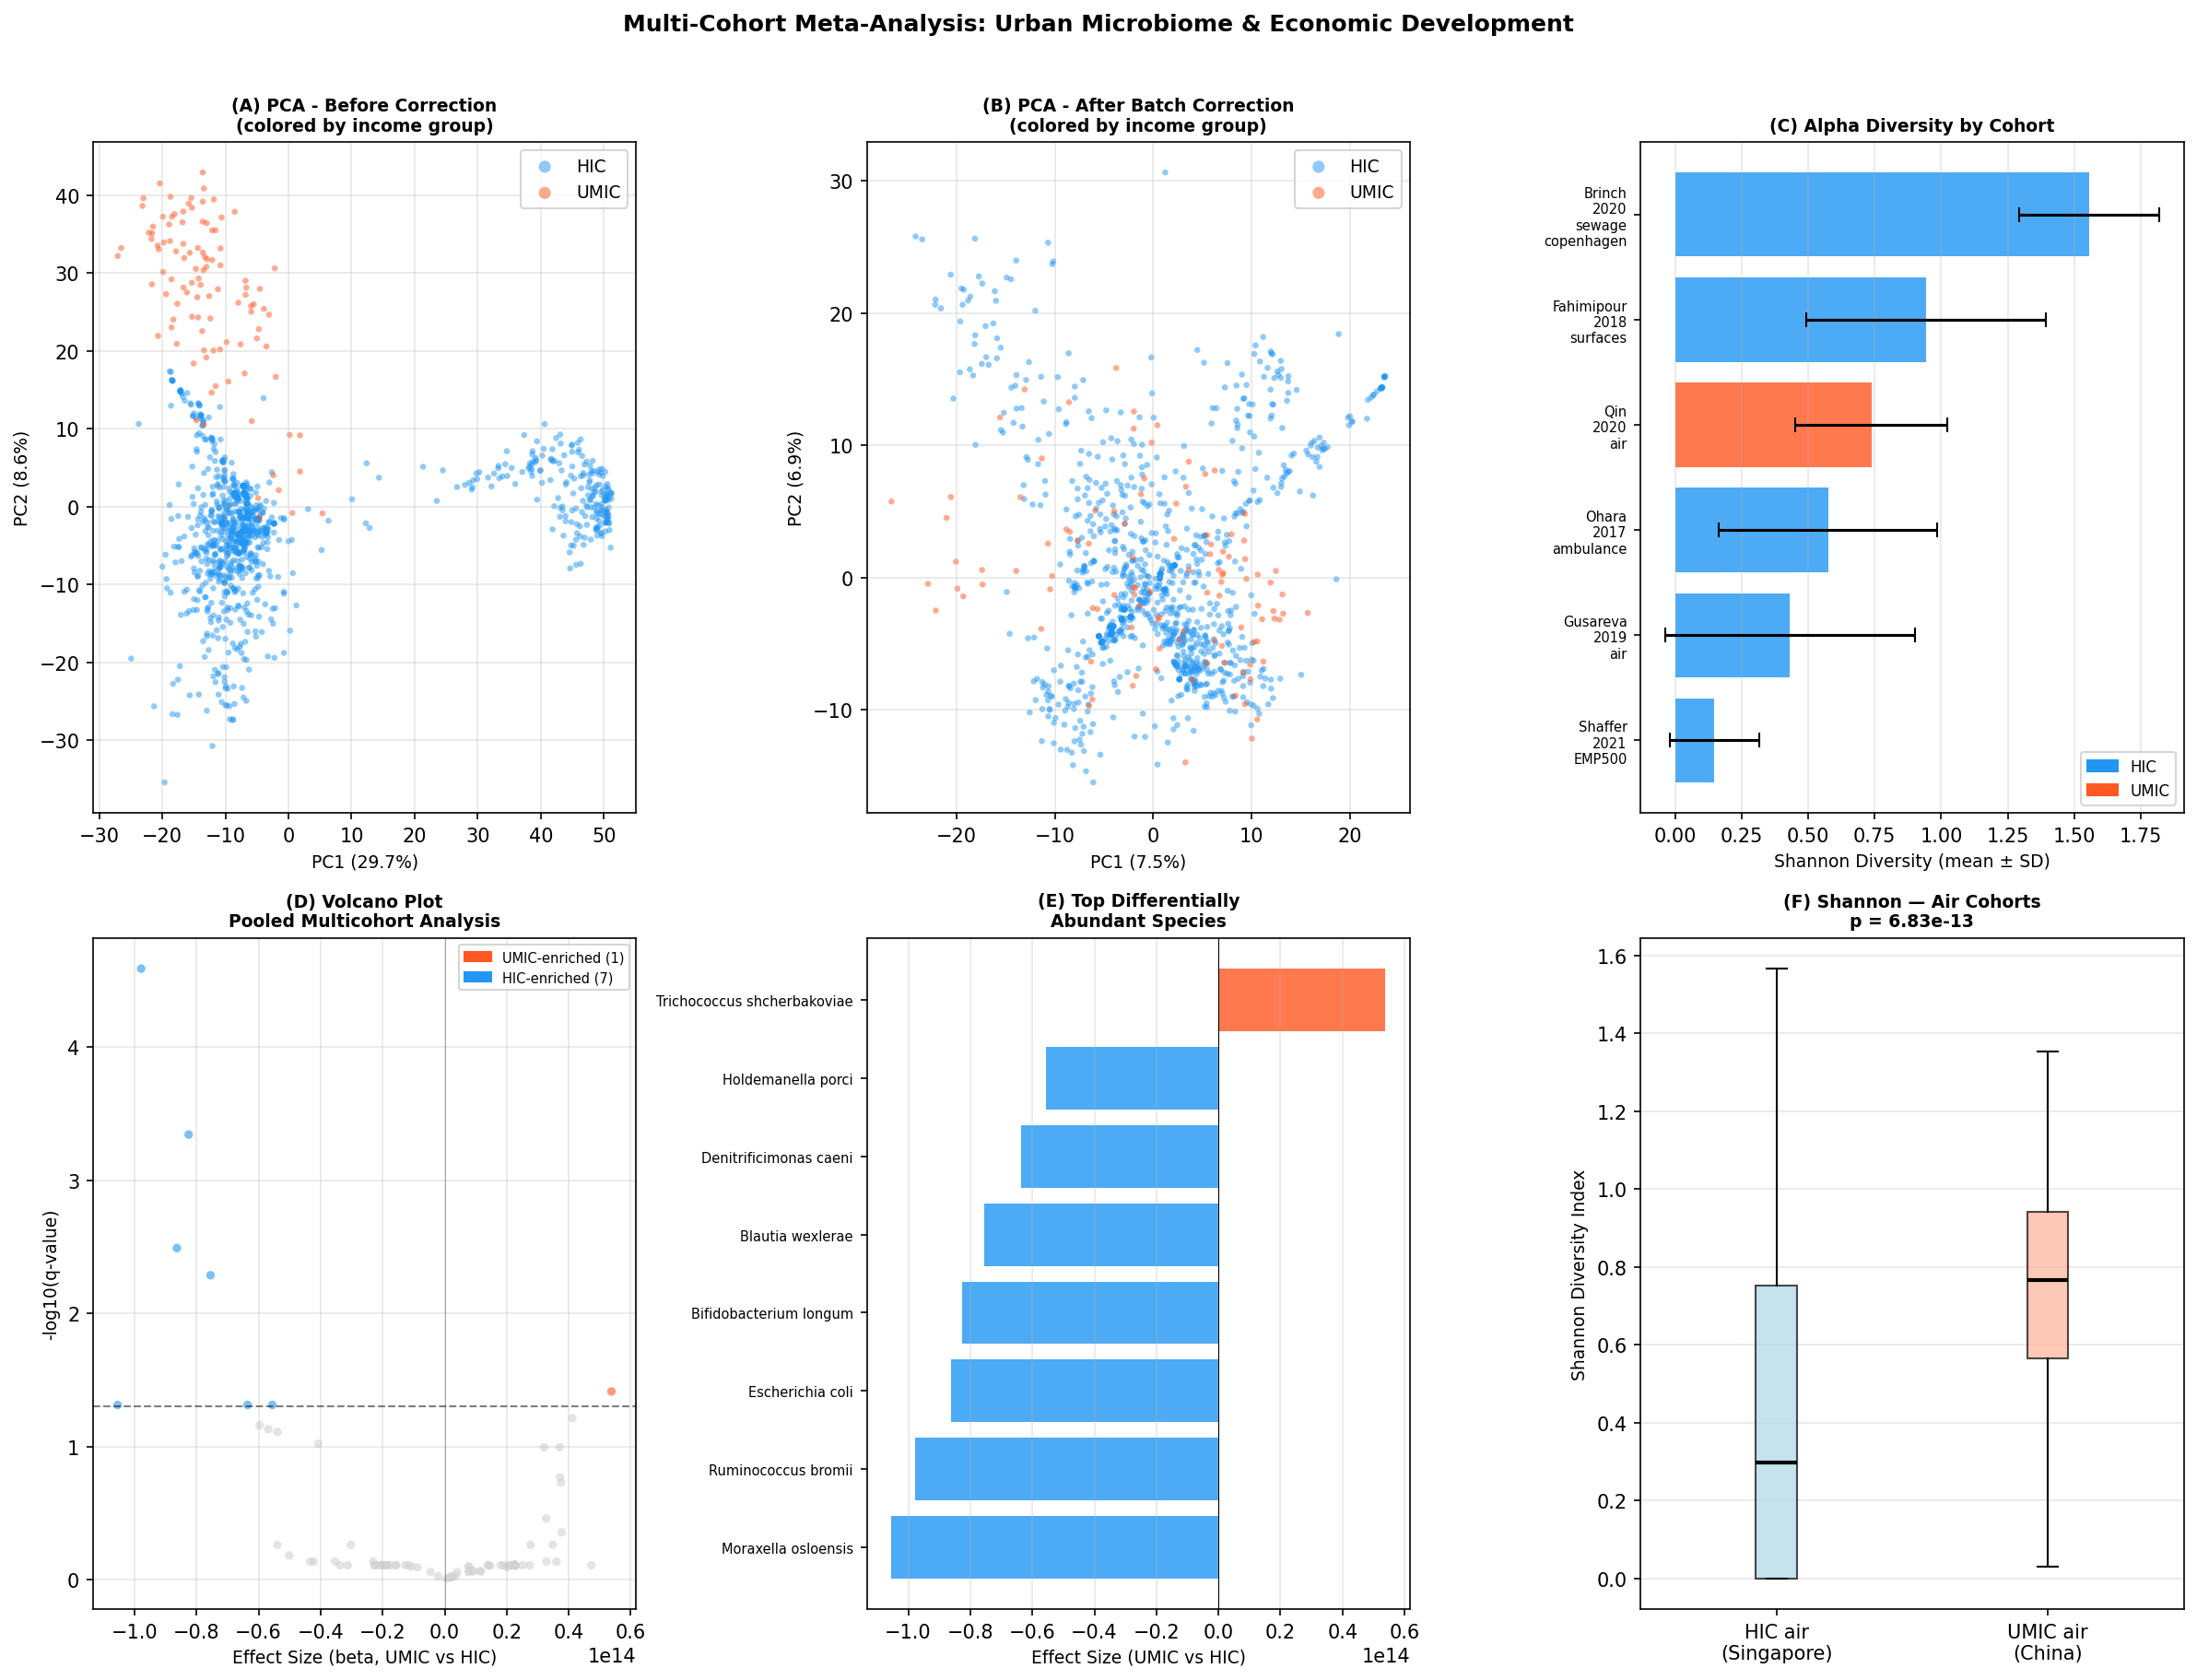
\includegraphics[width=1\textwidth,height=0.25\textheight,keepaspectratio]{output/meta_analysis/meta_analysis_main_figure.png}
\caption{\small Figure 1. Meta-analysis. (A-B) PCA before/after OLS batch correction (colored by income group): HIC blue, UMIC orange. Before correction cohorts separate; after correction income-group signal emerges. (C) Shannon diversity per cohort. (D) Volcano plot (pooled): 2 species survive FDR correction. (E) Top 15 species by effect size. (F) Shannon diversity in air cohorts only (Singapore HIC vs China UMIC): UMIC significantly higher ($p=6.8\times10^{-13}$).}
\label{fig:main}
\end{figure}

\begin{figure}[h!]
\centering
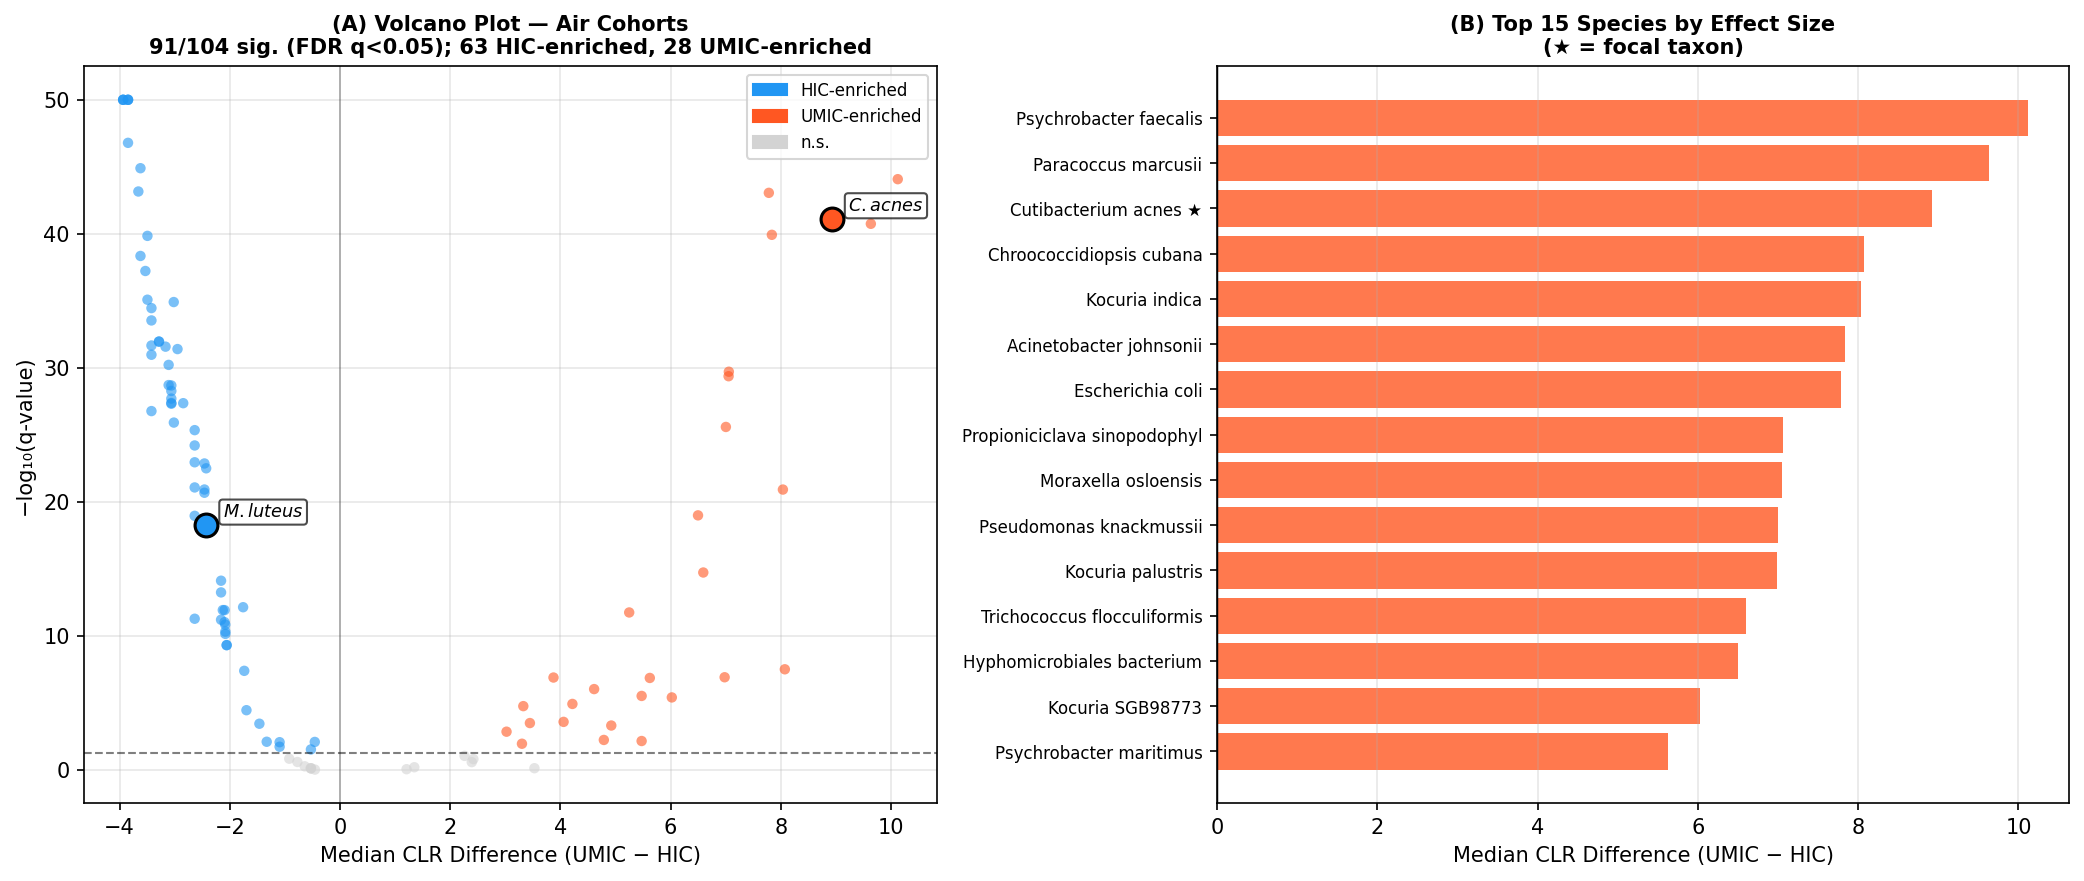
\includegraphics[width=0.98\textwidth,height=0.14\textheight,keepaspectratio]{output/meta_analysis/air_cohort_comparison_figure.png}
\caption{\small Figure 2. Air-cohort comparison (Gusareva 2019, Singapore vs.\ Qin 2020, China). (A) Volcano plot: 91/104 species differentially abundant (FDR $q<0.05$); 63 HIC-enriched (blue), 28 UMIC-enriched (orange). (B) Top 15 species by effect size.}
\label{fig:air}
\end{figure}

% ============================================================
\section*{Comparison with Published Data}

\textbf{Reference:} Danko et al.\ (2021), \href{https://www.cell.com/cell/fulltext/S0092-8674(21)00585-7}{``A global metagenomic map of urban microbiomes and antimicrobial resistance''}, Cell, (MetaSUB Consortium; 4728 samples, 60 cities).

\textbf{Alignment with our findings:} 
Both studies confirm that geography dominates urban microbiome variance over economic status, and that unadjusted cross-city comparisons are highly confounded. 
Both studies report globally prevalent taxa also detected in our air-cohort comparison: \textit{Micrococcus luteus} is HIC-enriched in our data ($q=5.7\times10^{-19}$), consistent with MetaSUB findings. \textit{Cutibacterium acnes} is UMIC-enriched in our air cohort ($q=8.0\times10^{-42}$), diverging from the MetaSUB pattern --- likely reflecting higher human-skin aerosol load in Chinese outdoor air.
The MetaSUB also found higher AMR gene prevalence in lower-income cities, consistent with the higher microbial diversity observed in UMIC environments.\\
\textbf{Analytical differences:}\\
1. Resistome profiling: AMR gene quantification linked income to public-health outcomes, absent from our analysis.\\
2. Standardised sampling: uniform surface swabs across cities eliminated material-type heterogeneity that limited our pooled result to 8 significant species.

\end{document}
